\documentclass[12pt,a4paper,twoside]{article}

\usepackage[a4paper,margin=1in]{geometry}
\usepackage{setspace}
\usepackage{graphicx}
\usepackage{array}
\usepackage{longtable}
\usepackage{booktabs}
\usepackage{fancyhdr}
\usepackage{titlesec}
\usepackage{enumitem}
\usepackage{xcolor}
\usepackage{tikz}
\usetikzlibrary{arrows.meta, positioning, shapes.geometric}
\usepackage[hidelinks]{hyperref}

% Screenshots resolve whether the folder structure is kept or flattened.
\graphicspath{{../screens/}{screens/}{./}}

\setstretch{1.5}

\pagestyle{fancy}
\fancyhf{}

\fancyhead[LO]{\small\textbf{BCA}}
\fancyhead[RE]{\small\textbf{Specialization Project}}

\fancyfoot[C]{\thepage}

\renewcommand{\headrulewidth}{0.4pt}

\titleformat{\section}
{\large\bfseries}
{\thesection.}
{0.5em}
{}

% Swatch helper for the colour palette tables
\newcommand{\swatch}[1]{\tikz[baseline=-0.6ex]\draw[fill=#1,draw=gray!50,rounded corners=1pt] (0,0) rectangle (0.62,0.32);}

\begin{document}

%%%%%%%%%%%%%%%%%%%%%%%%%%%%%%%%%%%%%%%%%%%%%%%%%%
% TITLE PAGE
%%%%%%%%%%%%%%%%%%%%%%%%%%%%%%%%%%%%%%%%%%%%%%%%%%

\begin{titlepage}
\thispagestyle{empty}

\begin{center}

{\Large\textbf{USER INTERFACE DESIGN DOCUMENT}}
\vspace{1cm}

{\Huge\textbf{Autonomous Video Ad-Placement \& Contextual Safety Analyzer}}\vspace{1.5cm}

Submitted in partial fulfillment of the requirements for the course

\vspace{0.5cm}

{\Large\textbf{Specialization Project}}

\vspace{1cm}

\textbf{Submitted By}

\vspace{0.5cm}

\begin{tabular}{ll}
Andrew Shelton S & 2441609\\
Akash Ganesh & 2441604\\
Andrew Judah & 2441608\\
Ramona Elisha Mary & 2441646\\
\end{tabular}

\vfill

\textbf{Under the Guidance of}\\[0.3cm]

Dr. Chanti\\
Assistant Professor

\vfill

Department of Computer Science\\
School of Sciences\\
CHRIST (Deemed to be University)\\
Bangalore

\vfill

Academic Year 2026--2027

\end{center}
\end{titlepage}

%%%%%%%%%%%%%%%%%%%%%%%%%%%%%%%%%%%%%%%%%%%%%%%%%%
% TABLE OF CONTENTS
%%%%%%%%%%%%%%%%%%%%%%%%%%%%%%%%%%%%%%%%%%%%%%%%%%

\tableofcontents
\newpage

%%%%%%%%%%%%%%%%%%%%%%%%%%%%%%%%%%%%%%%%%%%%%%%%%%
\section{Introduction}
%%%%%%%%%%%%%%%%%%%%%%%%%%%%%%%%%%%%%%%%%%%%%%%%%%

The purpose of this document is to describe the user interface design of the
\textbf{Autonomous Video Ad-Placement \& Contextual Safety Analyzer}, a locally hosted
desktop application that audits long-form video for brand-safety risks and identifies
premium advertisement placement surfaces. This document provides the screen layouts,
navigation flow, interface standards, validation rules, and design decisions that
govern the system's presentation layer.

The application is branded \textbf{AdSafe Studio} in the interface. Its visual design
deliberately follows the conventions of professional creator tooling --- a persistent
top bar, a left navigation rail, and a content table with inline status --- so that the
target users (video creators and marketing teams) encounter an interface whose
structure is already familiar to them.

All screen figures in this document are \textbf{live captures of the working
application}, not mockups. The interface is fully implemented and operational.

%%%%%%%%%%%%%%%%%%%%%%%%%%%%%%%%%%%%%%%%%%%%%%%%%%
\section{User Roles}
%%%%%%%%%%%%%%%%%%%%%%%%%%%%%%%%%%%%%%%%%%%%%%%%%%

\subsection{Usage Personas}

The system is a single-user desktop tool. The following personas describe the
\emph{usage contexts} the interface is designed to serve, as identified in the Software
Requirements Specification.

\begin{table}[htbp]
\centering
\begin{tabular}{|p{4cm}|p{8cm}|}
\hline
\textbf{Persona} & \textbf{Goals served by the interface}\\
\hline
Video Creator / Editor & Verify brand safety and monetization eligibility before
publishing; locate sponsor placement opportunities\\
\hline
Digital Marketing Agency & Rapidly audit creator content before attaching a client
brand; export evidence of the audit\\
\hline
Compliance Officer & Review flagged material against organisational policy; configure
the restricted keyword dictionary and detection thresholds\\
\hline
\end{tabular}
\end{table}

\subsection{Authentication: Deliberately Out of Scope}

The application does \textbf{not} implement user accounts, login, or role-based access
control, and no such screens exist. This is a considered design decision rather than an
omission:

\begin{itemize}[nosep]
\item The system is specified as an \textbf{offline, locally hosted} application. All
media and audit data remain on the operator's own machine and are never transmitted.
\item Introducing an authentication layer would add a credential store without adding
any security benefit, since access to the application already implies access to the
host filesystem on which its database and media reside.
\item The privacy objective in the SRS is satisfied by \emph{data never leaving the
machine}, not by access control within it.
\end{itemize}

Accordingly the personas above are not authenticated roles; every persona operates the
same single-user interface. Should the system later be deployed as a shared or
multi-tenant service, authentication and role separation would be introduced at that
point.

%%%%%%%%%%%%%%%%%%%%%%%%%%%%%%%%%%%%%%%%%%%%%%%%%%
\section{Navigation Structure}
%%%%%%%%%%%%%%%%%%%%%%%%%%%%%%%%%%%%%%%%%%%%%%%%%%

The application is a single-page application with client-side routing. A persistent
application shell (top bar and navigation rail) frames every screen, so the primary
destinations are reachable in one click from anywhere. The Upload dialog is modal and
can be invoked from any screen through the \textbf{Create} action.

\begin{figure}[htbp]
\centering
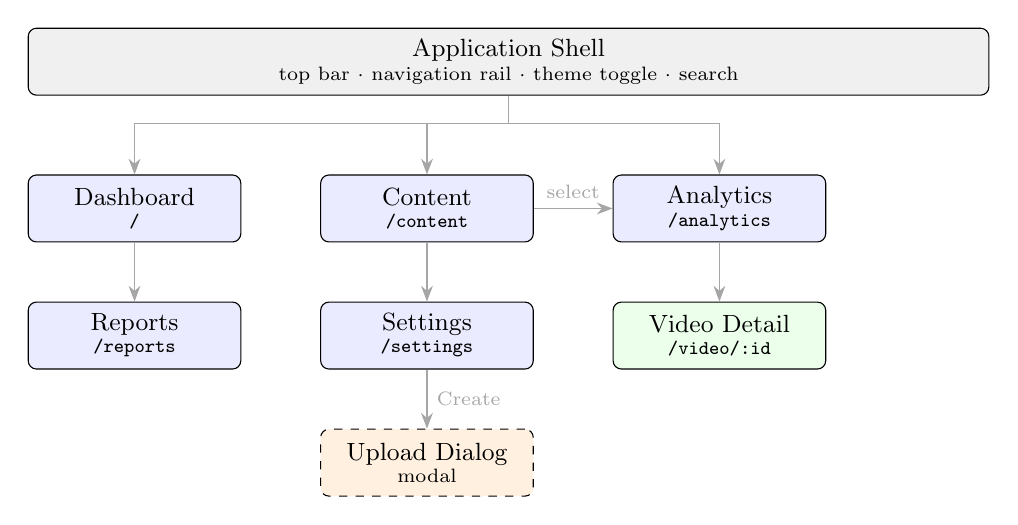
\begin{tikzpicture}[
  node distance=0.75cm and 1.0cm,
  box/.style={draw, rounded corners=3pt, minimum width=2.7cm, minimum height=0.85cm,
              align=center, font=\small},
  shell/.style={box, fill=gray!12, minimum width=12.2cm},
  prim/.style={box, fill=blue!8},
  sub/.style={box, fill=green!8},
  modal/.style={box, fill=orange!12, dashed},
  arr/.style={-{Stealth[length=2mm]}, gray!70}
]

\node[shell] (shell) {Application Shell\\[-2pt]{\scriptsize top bar $\cdot$ navigation rail $\cdot$ theme toggle $\cdot$ search}};

\node[prim, below=1.0cm of shell.south west, anchor=north west, xshift=0.0cm] (dash) {Dashboard\\[-3pt]{\scriptsize \texttt{/}}};
\node[prim, right=of dash] (content) {Content\\[-3pt]{\scriptsize \texttt{/content}}};
\node[prim, right=of content] (analytics) {Analytics\\[-3pt]{\scriptsize \texttt{/analytics}}};
\node[prim, below=0.75cm of dash] (reports) {Reports\\[-3pt]{\scriptsize \texttt{/reports}}};
\node[prim, below=0.75cm of content] (settings) {Settings\\[-3pt]{\scriptsize \texttt{/settings}}};

\node[sub, below=0.75cm of analytics] (detail) {Video Detail\\[-3pt]{\scriptsize \texttt{/video/:id}}};
\node[modal, below=0.75cm of settings] (upload) {Upload Dialog\\[-3pt]{\scriptsize modal}};

\draw[arr] (shell.south) -- ++(0,-0.35) -| (dash.north);
\draw[arr] (shell.south) -- ++(0,-0.35) -| (content.north);
\draw[arr] (shell.south) -- ++(0,-0.35) -| (analytics.north);
\draw[arr] (dash.south) -- (reports.north);
\draw[arr] (content.south) -- (settings.north);
\draw[arr] (content.east) -- node[above, font=\scriptsize] {select} (analytics.west);
\draw[arr] (analytics.south) -- (detail.north);
\draw[arr] (settings.south) -- node[right, font=\scriptsize] {Create} (upload.north);

\end{tikzpicture}
\caption{System Navigation Flow. Blue: primary destinations in the navigation rail.
Green: contextual screen reached by selecting a video. Orange (dashed): modal overlay
invokable from any screen.}
\end{figure}

\noindent Secondary navigation paths:

\begin{itemize}[nosep]
\item Dashboard $\rightarrow$ Video Detail (via the \emph{Recent uploads} list)
\item Dashboard $\rightarrow$ Analytics (via \emph{See full analytics})
\item Video Detail $\rightarrow$ Reports (report generated directly from the detail header)
\item Any screen $\rightarrow$ Dashboard (via the application logo)
\end{itemize}

%%%%%%%%%%%%%%%%%%%%%%%%%%%%%%%%%%%%%%%%%%%%%%%%%%
\section{User Interface Standards}
%%%%%%%%%%%%%%%%%%%%%%%%%%%%%%%%%%%%%%%%%%%%%%%%%%

\subsection{Typography}

A single typeface is used throughout. Weight and size, not font family, carry the
visual hierarchy.

\begin{table}[htbp]
\centering
\begin{tabular}{|p{4cm}|p{3.2cm}|p{4.4cm}|}
\hline
\textbf{Element} & \textbf{Font} & \textbf{Specification}\\
\hline
Page title & Roboto Regular & 25\,px / weight 400\\
\hline
Section heading & Roboto Medium & 15\,px / weight 500\\
\hline
Body text & Roboto Regular & 14\,px / weight 400\\
\hline
Secondary text & Roboto Regular & 12--13\,px, muted colour\\
\hline
Button label & Roboto Medium & 14\,px / weight 500\\
\hline
Statistic value & Roboto Regular & 32\,px / weight 400\\
\hline
Icons & Material Symbols & Outlined, 20--24\,px\\
\hline
\end{tabular}
\end{table}

\subsection{Colour Palette}

The interface ships a \textbf{dark theme by default} with a light theme available via a
toggle in the top bar. Colour values were selected against measured contrast rather
than by eye.

\subsubsection*{Surfaces and text}

\begin{table}[htbp]
\centering
\begin{tabular}{|p{3.3cm}|p{2.6cm}|p{2.6cm}|p{3.0cm}|}
\hline
\textbf{Role} & \textbf{Dark} & \textbf{Light} & \textbf{Contrast (dark)}\\
\hline
Page background & \swatch{black!94} \texttt{\#0F0F0F} & \swatch{black!2} \texttt{\#F9F9F9} & ---\\
\hline
Surface (cards) & \swatch{black!87} \texttt{\#212121} & \swatch{white} \texttt{\#FFFFFF} & ---\\
\hline
Primary text & \swatch{black!6} \texttt{\#F1F1F1} & \swatch{black!94} \texttt{\#0F0F0F} & 14.26:1\\
\hline
Secondary text & \swatch{black!33} \texttt{\#AAAAAA} & \swatch{black!62} \texttt{\#606060} & 6.93:1\\
\hline
Action / primary & \swatch{blue!65} \texttt{\#3EA6FF} & \swatch{blue!80!black} \texttt{\#065FD4} & 6.21:1\\
\hline
Accent (brand) & \swatch{red!85} \texttt{\#FF4E45} & \swatch{red!75!black} \texttt{\#CC0000} & 4.93:1\\
\hline
\end{tabular}
\end{table}

\noindent\textbf{Note on the action colour.} The light-theme blue \texttt{\#065FD4}
measures only \textbf{2.76:1} against the dark card surface, which fails the WCAG~2.1
minimum of 3:1 for user-interface components. The dark theme therefore substitutes
\texttt{\#3EA6FF} (6.21:1). The action colour is a themed token rather than a fixed
value for this reason.

\subsubsection*{Status palette (fixed across both themes)}

Severity colours are held constant in both themes so that a given risk level always
reads identically. Each is verified at $\geq$3:1 against both surfaces, and the worst
adjacent pair separates by $\Delta E = 16.4$ under simulated deuteranopia (target
$\geq$12), so the palette remains distinguishable to colour-blind users.

\begin{table}[htbp]
\centering
\begin{tabular}{|p{3.6cm}|p{2.8cm}|p{5.4cm}|}
\hline
\textbf{Meaning} & \textbf{Value} & \textbf{Applied to}\\
\hline
High severity & \swatch{red!70!black} \texttt{\#D03B3B} & High-risk speech, weapon detections\\
\hline
Medium severity & \swatch{orange!70} \texttt{\#EC835A} & Medium-risk speech, substances\\
\hline
Low severity & \swatch{yellow!80!orange} \texttt{\#FAB219} & Low-risk speech\\
\hline
Positive / opportunity & \swatch{green!60!black} \texttt{\#0CA30C} & Ad spots, monetizable verdict\\
\hline
Limited monetization & \swatch{orange!80!yellow} \texttt{\#F5A623} & Restricted verdict badge\\
\hline
\end{tabular}
\end{table}

\noindent Colour is never the sole carrier of meaning. Every severity indicator pairs
its colour with a text label, and every status icon pairs with descriptive text.

\subsection{Layout and Components}

\begin{itemize}[nosep]
\item \textbf{Grid:} fixed 240\,px navigation rail; fluid content column capped at
1400\,px.
\item \textbf{Elevation:} a three-step surface ladder (page $\rightarrow$ surface
$\rightarrow$ raised) separated by 1\,px borders. Dark interfaces separate by border,
not shadow.
\item \textbf{Radius:} 12\,px cards, 18\,px pill buttons, 8\,px inputs, 999\,px chips.
\item \textbf{Spacing:} 4\,px base unit; 24\,px between major blocks.
\item \textbf{Feedback:} inline progress bars for long operations; transient snackbar
confirmations; skeleton placeholders while loading.
\end{itemize}

%%%%%%%%%%%%%%%%%%%%%%%%%%%%%%%%%%%%%%%%%%%%%%%%%%
\section{Screen Design}
%%%%%%%%%%%%%%%%%%%%%%%%%%%%%%%%%%%%%%%%%%%%%%%%%%

Seven screens comprise the interface. Each is described by its purpose, its constituent
components, and a capture of the implemented screen.

%%%%%%%%%%%%%%%%%%%%%%%%%%%%%%%%%%%%%%%%%%%%%%%%%%
\subsection{Dashboard Screen}
%%%%%%%%%%%%%%%%%%%%%%%%%%%%%%%%%%%%%%%%%%%%%%%%%%

\subsubsection*{Purpose}

Landing screen. Summarises the state of the entire library so the operator can judge
overall monetization health at a glance and resume recent work.

\subsubsection*{Components}

\begin{itemize}[nosep]
\item Four summary statistic cards --- videos in library, fully monetizable count,
total risk flags, total advertisement inventory
\item Library health panel with a proportional monetizable / restricted split bar
\item Recent uploads list with per-video status icons
\item Shortcut links to Analytics and Content
\item Empty state guiding a first-time user to upload
\end{itemize}

\begin{figure}[htbp]
\centering
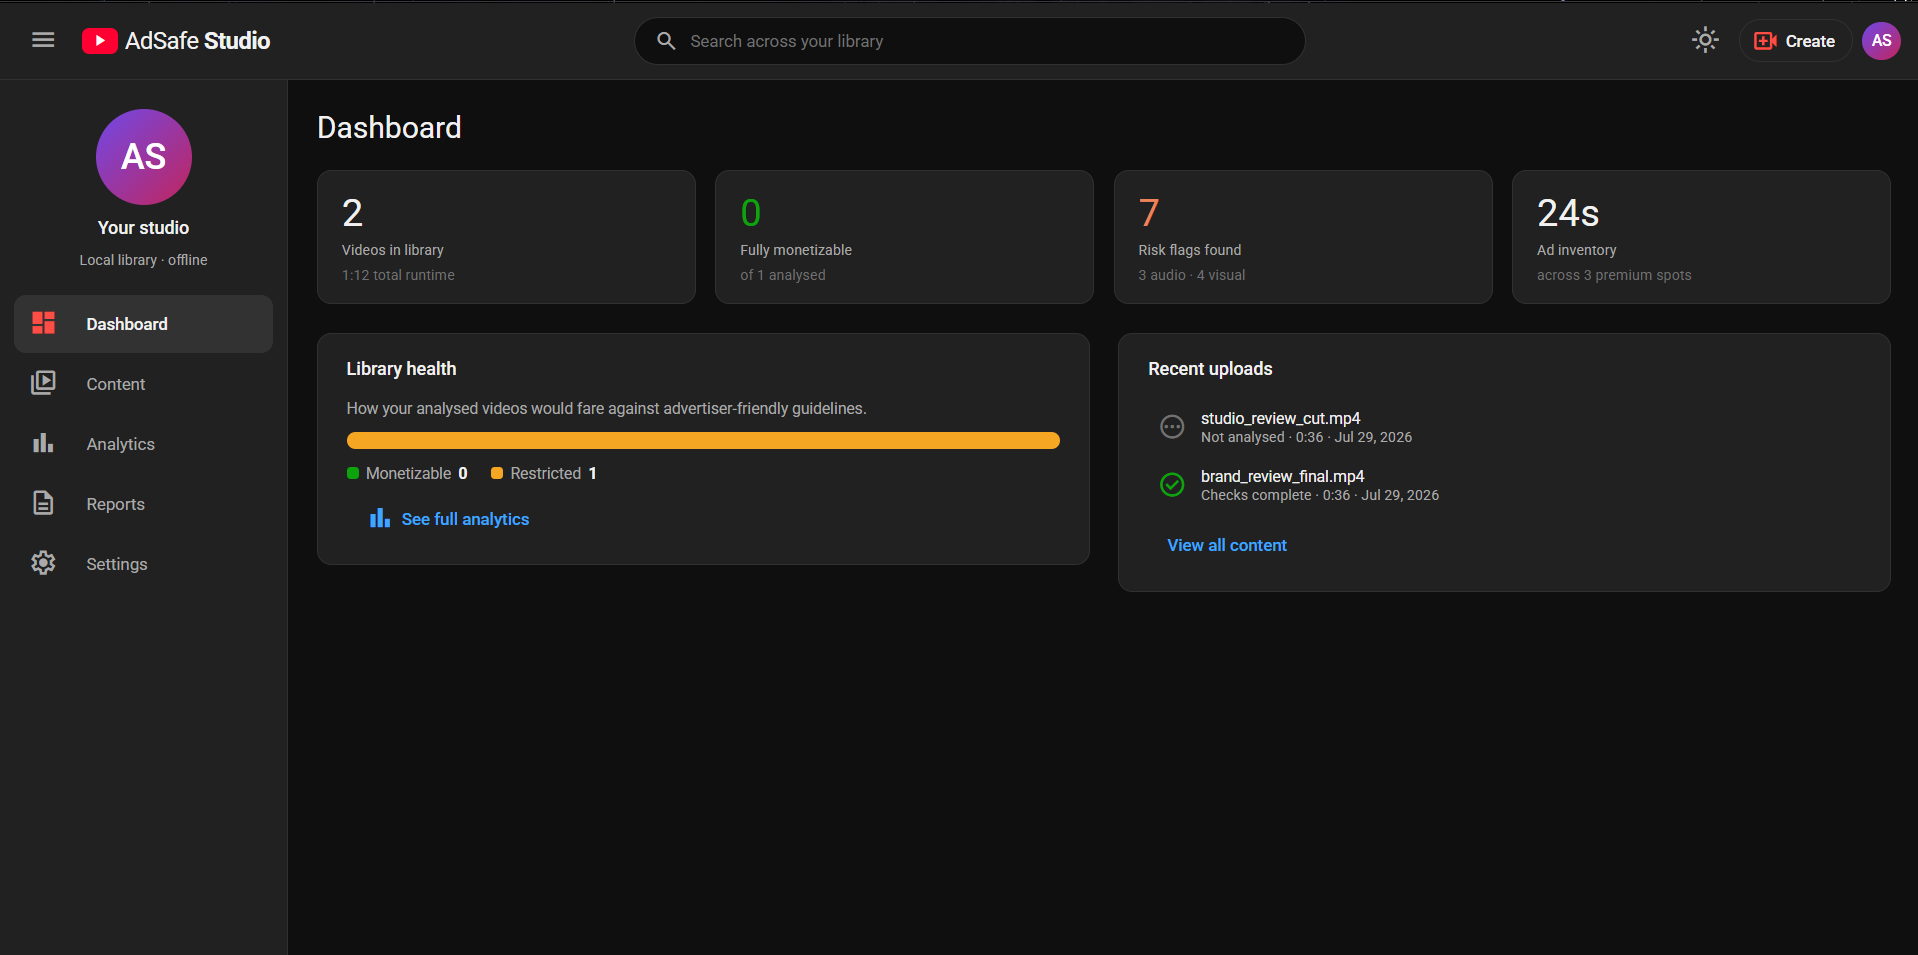
\includegraphics[width=\textwidth]{01-dashboard.png}
\caption{Dashboard Screen}
\end{figure}

\clearpage

%%%%%%%%%%%%%%%%%%%%%%%%%%%%%%%%%%%%%%%%%%%%%%%%%%
\subsection{Content Screen}
%%%%%%%%%%%%%%%%%%%%%%%%%%%%%%%%%%%%%%%%%%%%%%%%%%

\subsubsection*{Purpose}

The video library. Lists every ingested video with its monetization verdict and
analysis status, and is the launch point for running checks.

\subsubsection*{Components}

\begin{itemize}[nosep]
\item Sortable table: thumbnail, filename, technical metadata, monetization badge,
status, upload date, duration, flag counts, advertisement spot count
\item Monetization badge --- green currency icon (monetizable), amber (limited),
grey (not yet analysed)
\item Per-row hover actions: open, run/re-run checks, delete
\item Live progress bar with stage label while analysis runs
\item Filter bar and library-wide search
\item Empty state with a demo-video shortcut
\end{itemize}

\begin{figure}[htbp]
\centering
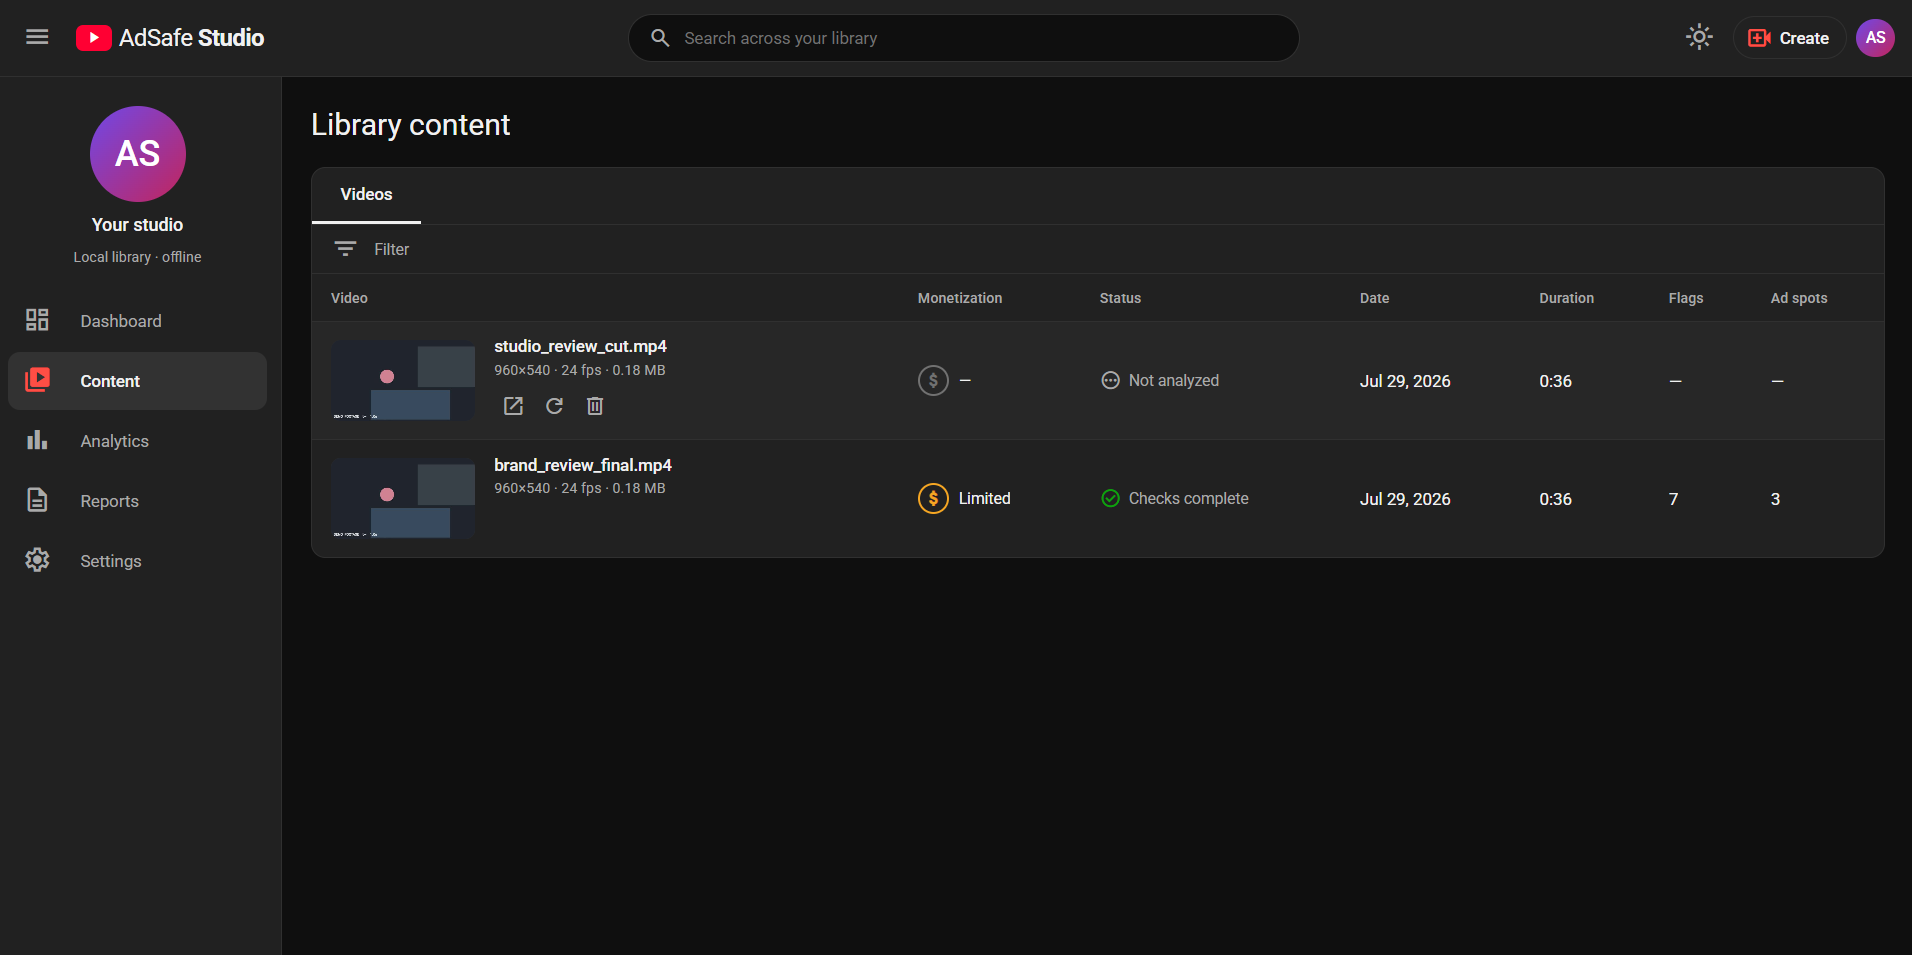
\includegraphics[width=\textwidth]{02-content.png}
\caption{Content Screen}
\end{figure}

\clearpage

%%%%%%%%%%%%%%%%%%%%%%%%%%%%%%%%%%%%%%%%%%%%%%%%%%
\subsection{Video Detail Screen}
%%%%%%%%%%%%%%%%%%%%%%%%%%%%%%%%%%%%%%%%%%%%%%%%%%

\subsubsection*{Purpose}

The primary analysis workspace. Presents every finding for a single video on a common
timeline synchronised with video playback.

\subsubsection*{Components}

\begin{itemize}[nosep]
\item Header with filename, monetization verdict badge, and export actions
\item Four statistic cards --- audio flags, visual risks, premium advertisement spots,
advertisement inventory
\item \textbf{Audit timeline:} three lanes (audio, visual, advertisement spots) with
colour-coded events, minute:second axis, and a live playhead. Events are clickable and
keyboard-operable; selecting one seeks the player to that moment
\item Embedded video player with native controls
\item Tabbed result tables --- audio flags (word, severity, transcript context),
visual risks (object, category, confidence, bounding box), advertisement spots
(interval, surface type, area, suitability)
\item Metadata panel
\end{itemize}

\begin{figure}[htbp]
\centering
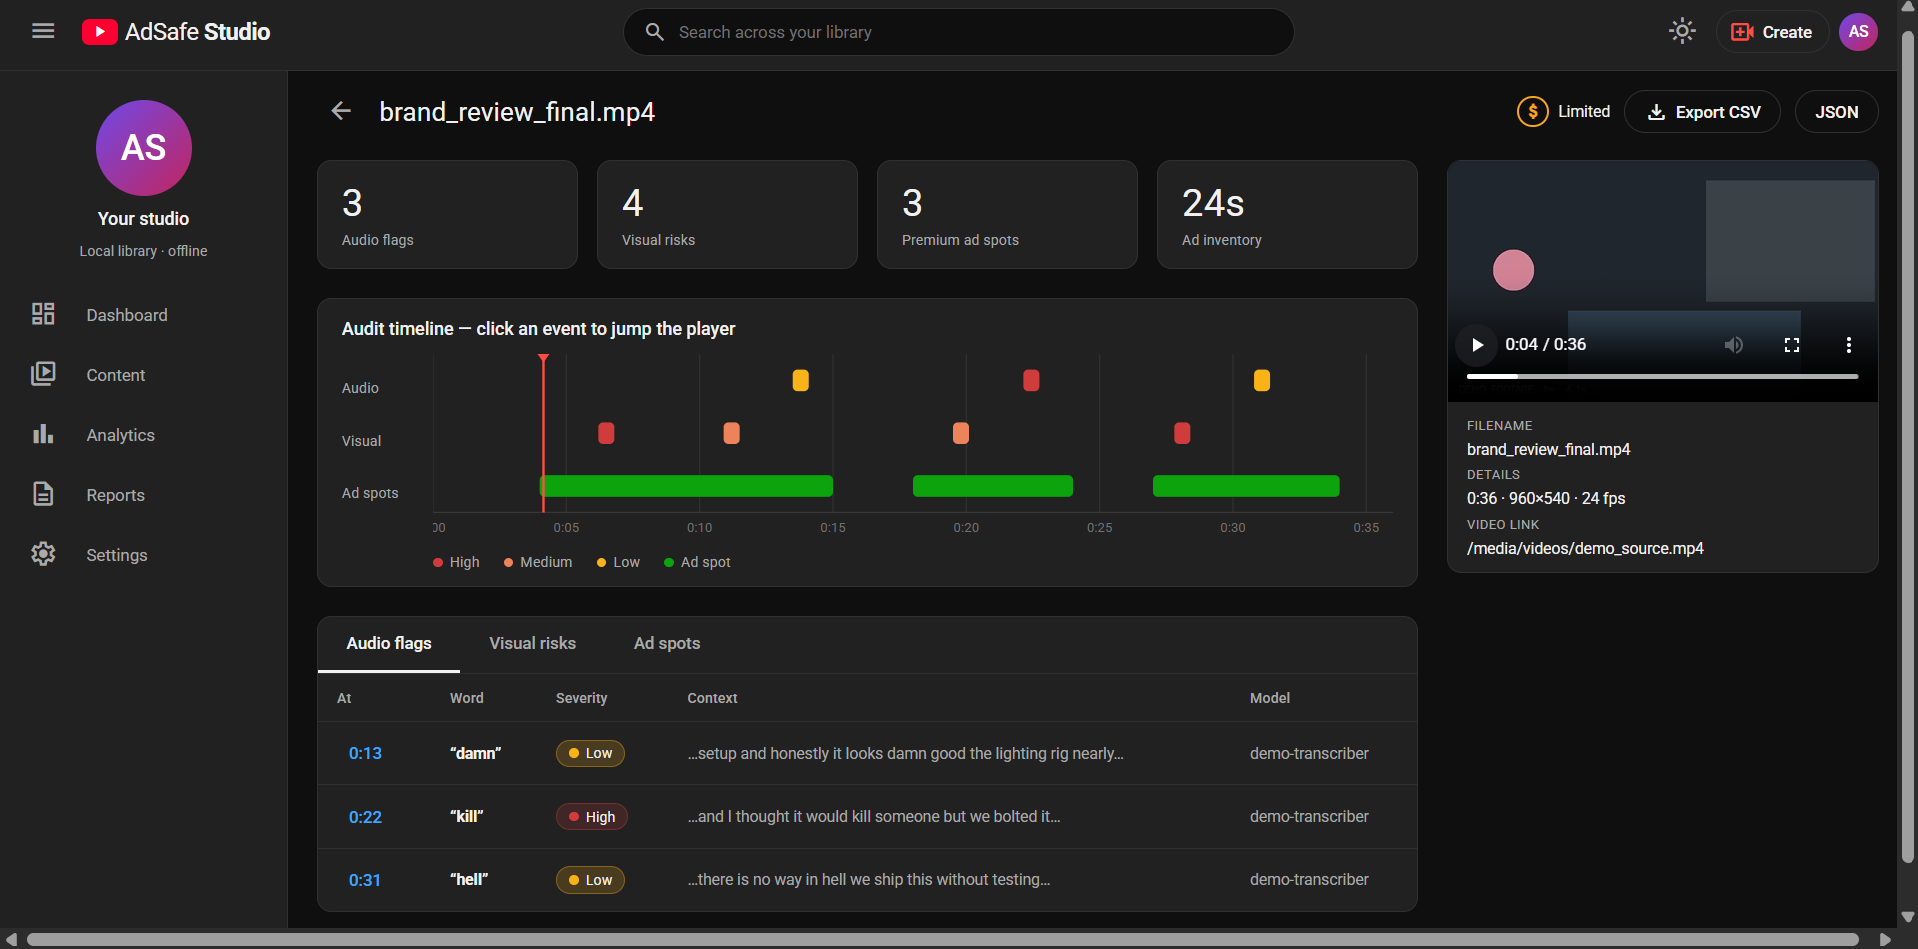
\includegraphics[width=\textwidth]{03-video-detail.png}
\caption{Video Detail Screen, showing the audit timeline synchronised with playback}
\end{figure}

\clearpage

%%%%%%%%%%%%%%%%%%%%%%%%%%%%%%%%%%%%%%%%%%%%%%%%%%
\subsection{Analytics Screen}
%%%%%%%%%%%%%%%%%%%%%%%%%%%%%%%%%%%%%%%%%%%%%%%%%%

\subsubsection*{Purpose}

Aggregates findings across every analysed video, revealing recurring risks that are not
visible when inspecting one video at a time.

\subsubsection*{Components}

\begin{itemize}[nosep]
\item Three summary statistic cards
\item Monetization outcome split bar
\item Audio flags by severity (status palette)
\item Visual risks by category
\item Most frequently flagged words
\item Most frequently detected objects
\item Advertisement inventory by surface type, in seconds
\end{itemize}

\noindent Each chart prints its numeric value beside every bar, so the visualisation
also serves as its own data table.

\begin{figure}[htbp]
\centering
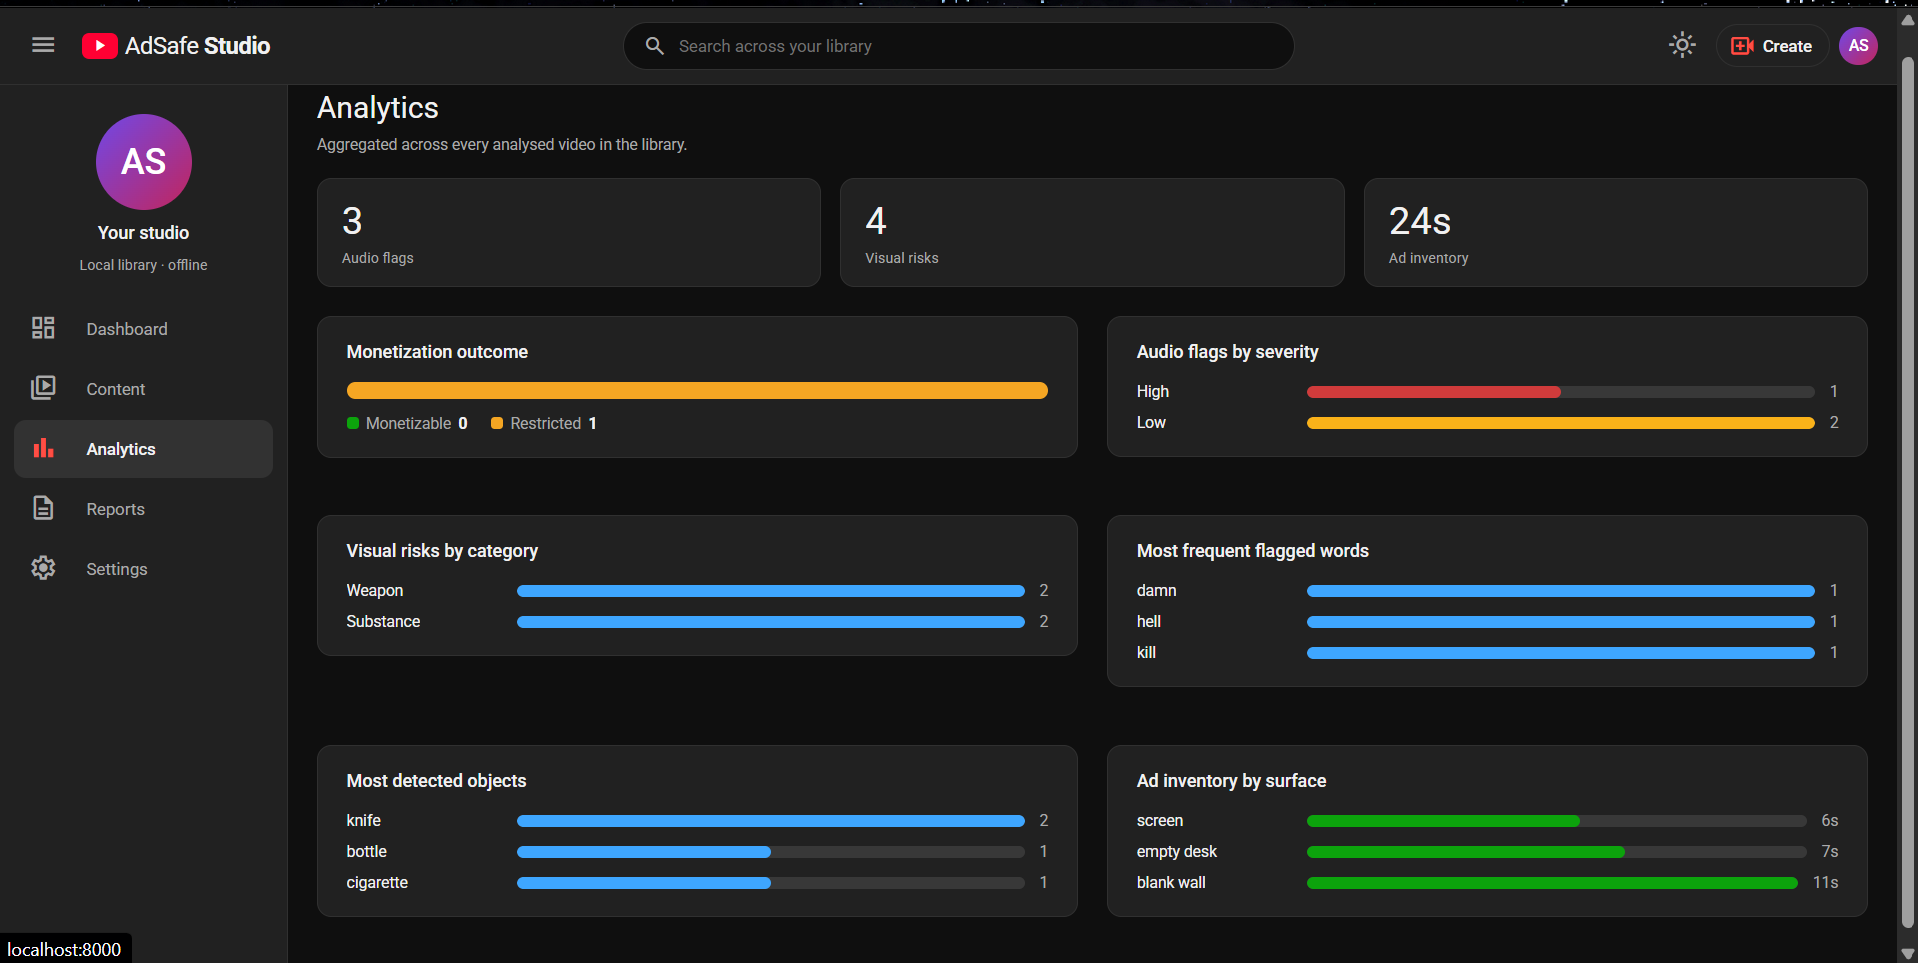
\includegraphics[width=\textwidth]{04-analytics.png}
\caption{Analytics Screen}
\end{figure}

\clearpage

%%%%%%%%%%%%%%%%%%%%%%%%%%%%%%%%%%%%%%%%%%%%%%%%%%
\subsection{Reports Screen}
%%%%%%%%%%%%%%%%%%%%%%%%%%%%%%%%%%%%%%%%%%%%%%%%%%

\subsubsection*{Purpose}

Generates and archives formal compliance reports for individual videos.

\subsubsection*{Components}

\begin{itemize}[nosep]
\item Video selector, restricted to analysed videos
\item Output format selector --- CSV, JSON
\item Generate action
\item Report history table --- generation timestamp, source video, format, risk totals,
compliance verdict
\item Per-row download action
\end{itemize}

\begin{figure}[htbp]
\centering
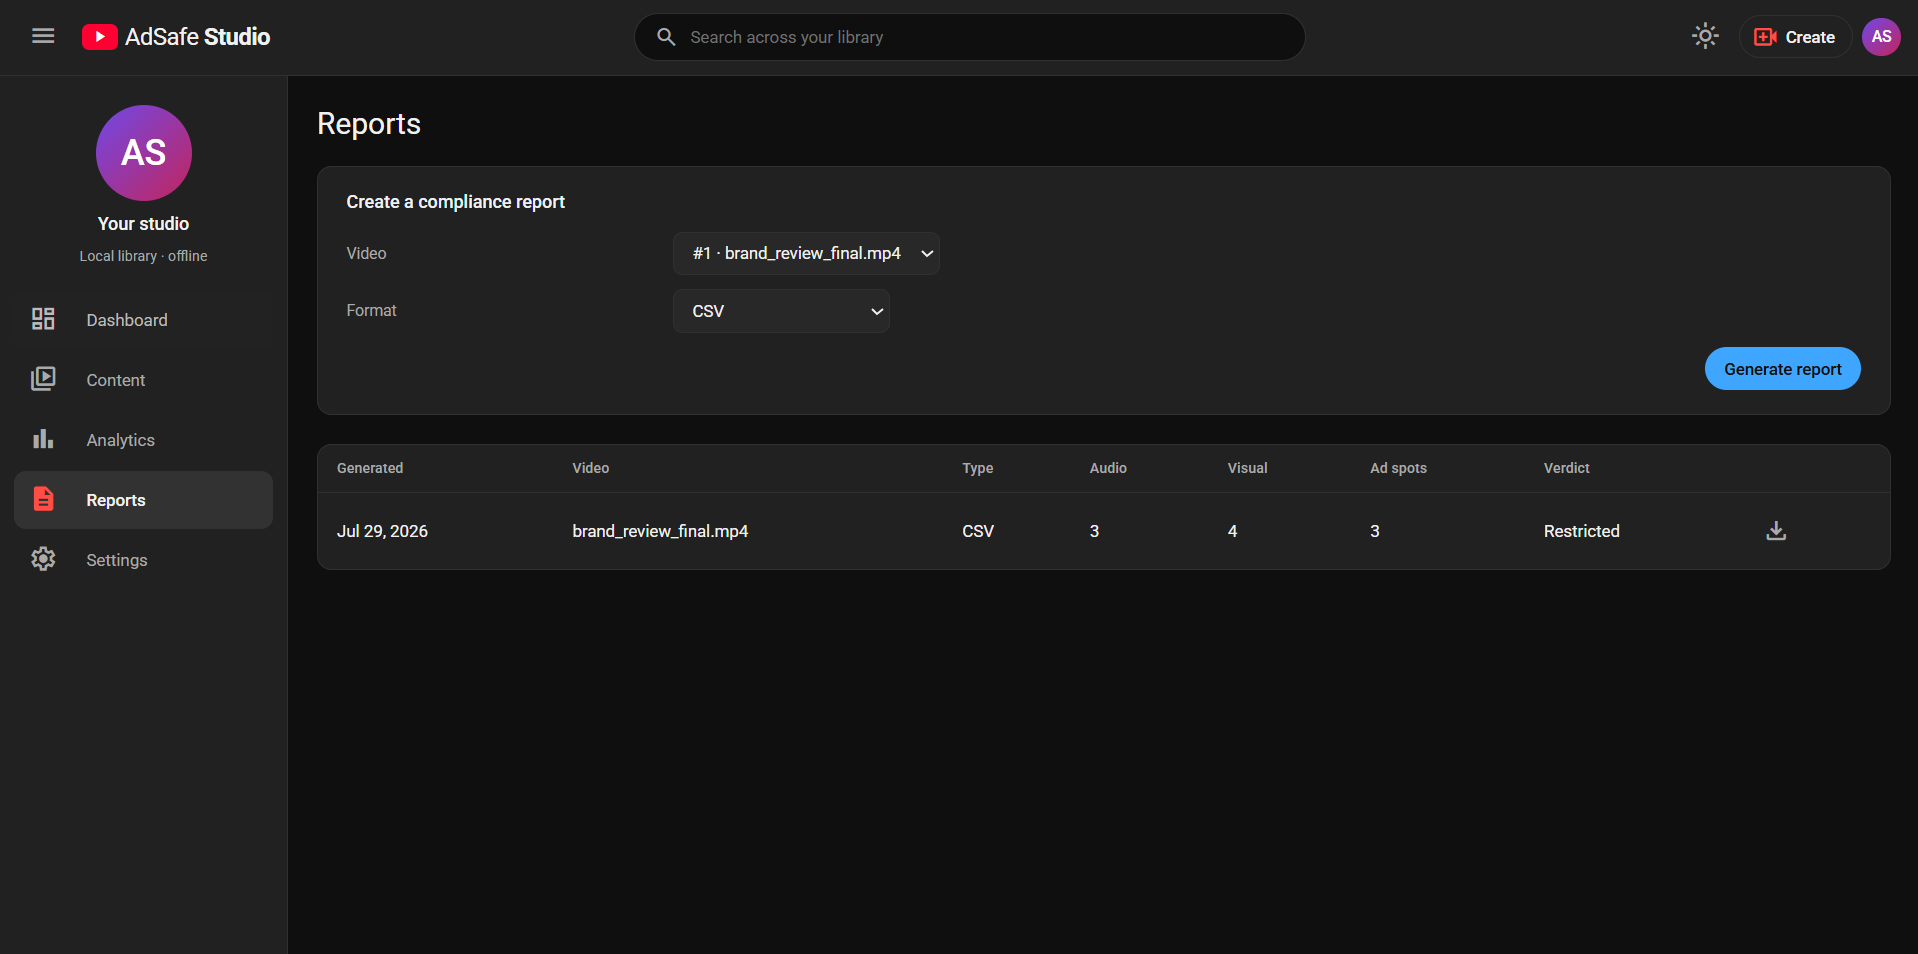
\includegraphics[width=\textwidth]{05-reports.png}
\caption{Reports Screen}
\end{figure}

\clearpage

%%%%%%%%%%%%%%%%%%%%%%%%%%%%%%%%%%%%%%%%%%%%%%%%%%
\subsection{Settings Screen}
%%%%%%%%%%%%%%%%%%%%%%%%%%%%%%%%%%%%%%%%%%%%%%%%%%

\subsubsection*{Purpose}

Configures detection behaviour. Changes are persisted and applied to subsequent
analysis runs.

\subsubsection*{Components}

\begin{itemize}[nosep]
\item Editable restricted keyword dictionary --- term and severity per row, with add
and remove actions
\item Pipeline parameters --- frame sample rate, minimum advertisement spot
persistence, detection confidence threshold
\item Transcription model selector
\item Save action, disabled while any field is invalid
\item Inline validation messages against the offending field
\end{itemize}

\begin{figure}[htbp]
\centering
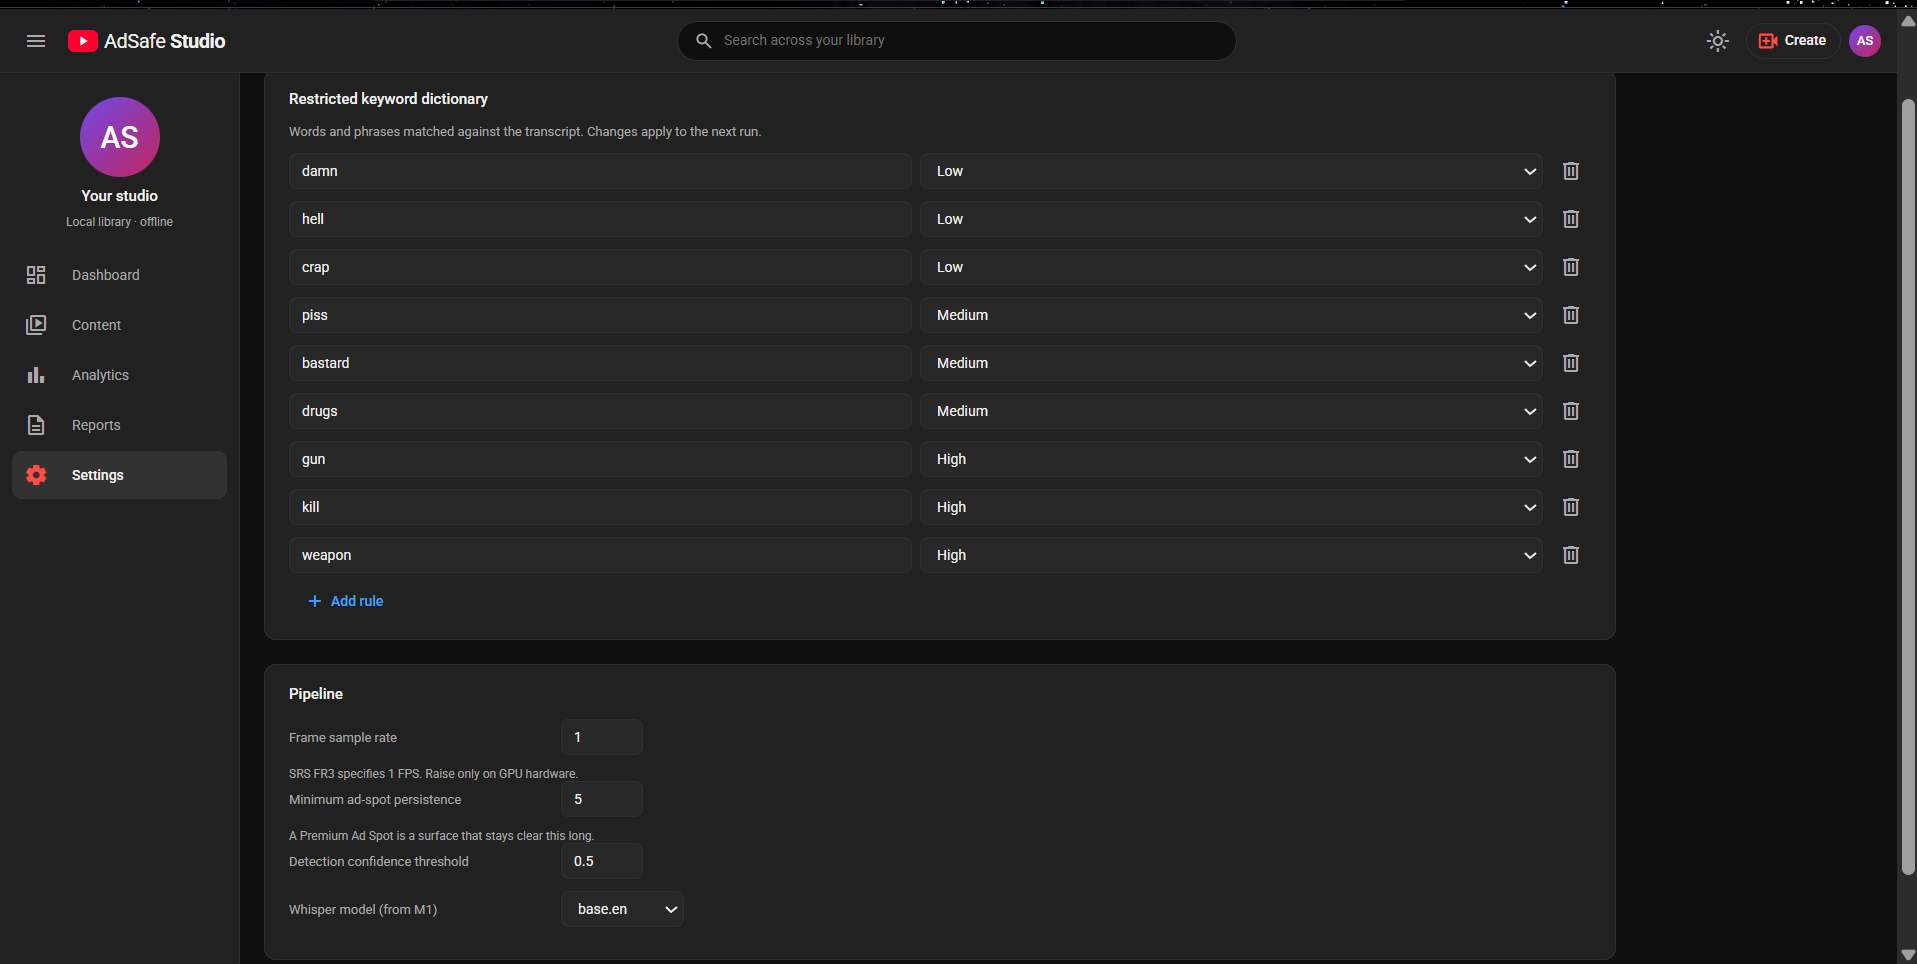
\includegraphics[width=\textwidth]{06-settings.png}
\caption{Settings Screen}
\end{figure}

\clearpage

%%%%%%%%%%%%%%%%%%%%%%%%%%%%%%%%%%%%%%%%%%%%%%%%%%
\subsection{Upload Dialog}
%%%%%%%%%%%%%%%%%%%%%%%%%%%%%%%%%%%%%%%%%%%%%%%%%%

\subsubsection*{Purpose}

Modal overlay for ingesting a video. Reachable from any screen via the \textbf{Create}
action.

\subsubsection*{Components}

\begin{itemize}[nosep]
\item Drag-and-drop zone with an equivalent file-picker button
\item Accepted-format and size guidance
\item Privacy reassurance stating that media never leaves the machine
\item Determinate upload progress bar
\item Inline validation message for rejected files
\item Dismiss action, disabled during transfer to prevent interruption
\end{itemize}

\begin{figure}[htbp]
\centering
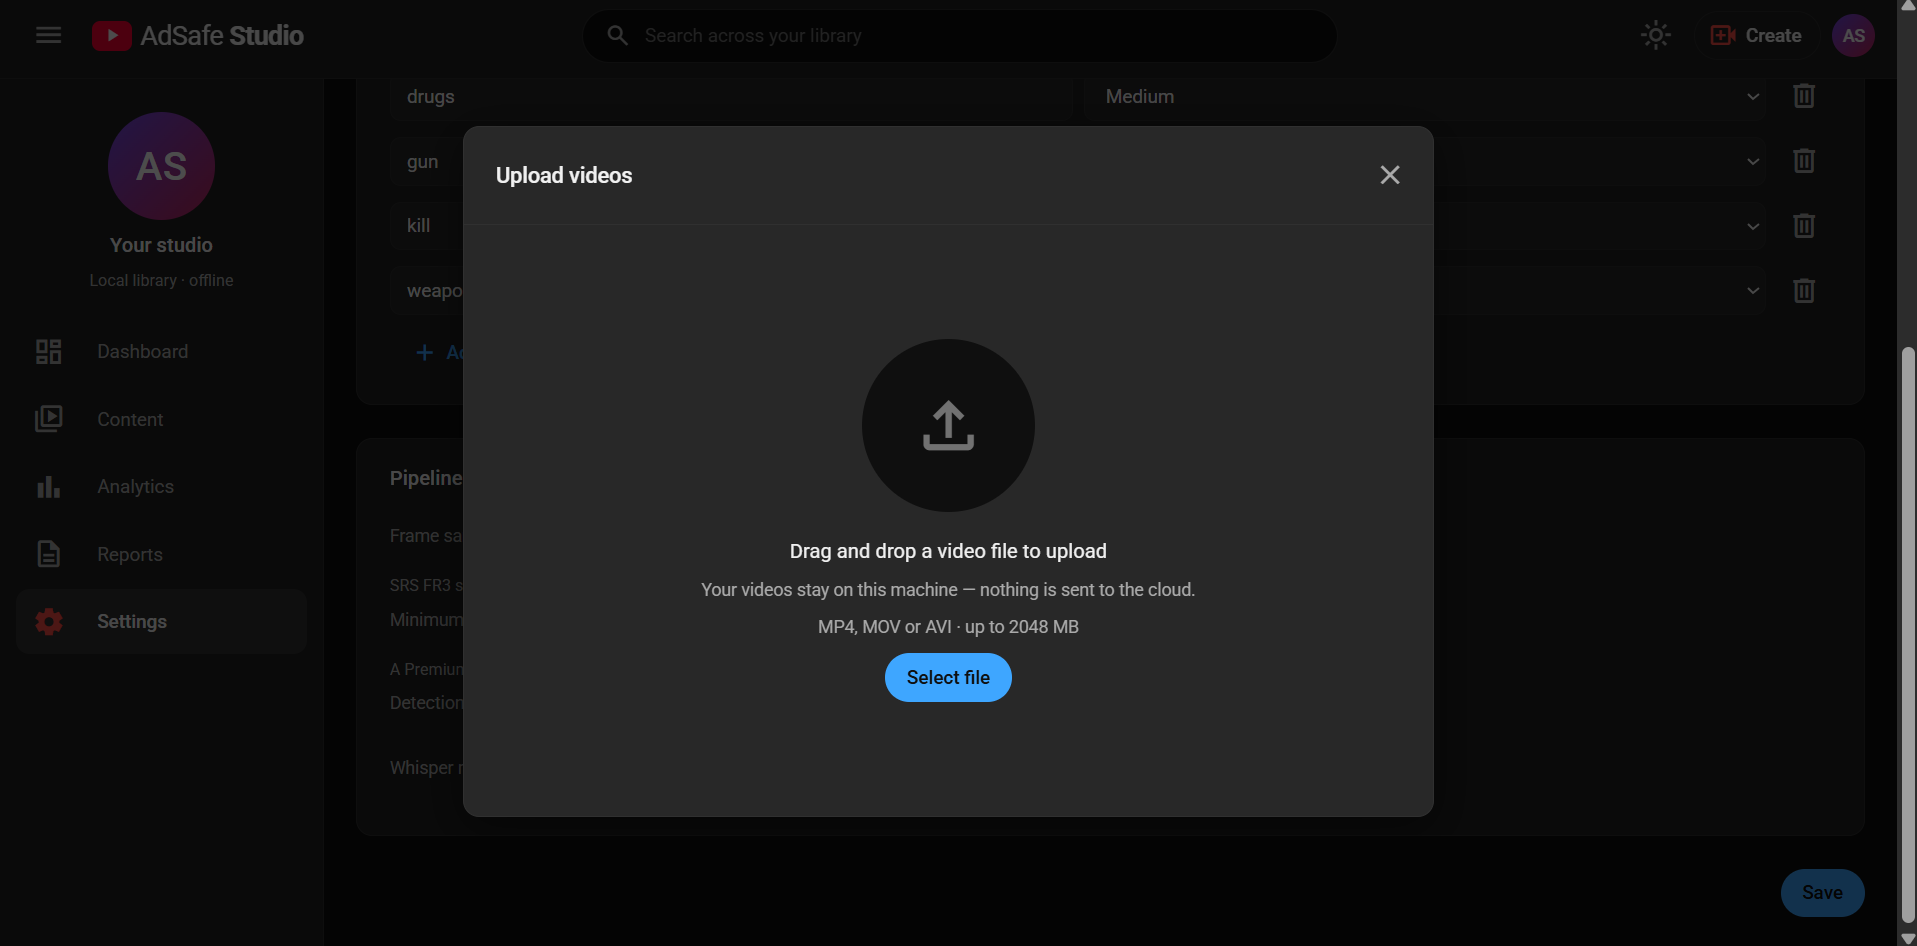
\includegraphics[width=0.92\textwidth]{07-upload-dialog.png}
\caption{Upload Dialog}
\end{figure}

\clearpage

%%%%%%%%%%%%%%%%%%%%%%%%%%%%%%%%%%%%%%%%%%%%%%%%%%
\subsection{Interaction States}
%%%%%%%%%%%%%%%%%%%%%%%%%%%%%%%%%%%%%%%%%%%%%%%%%%

Two states warrant illustration because they define how the interface communicates
progress and error.

\begin{figure}[htbp]
\centering
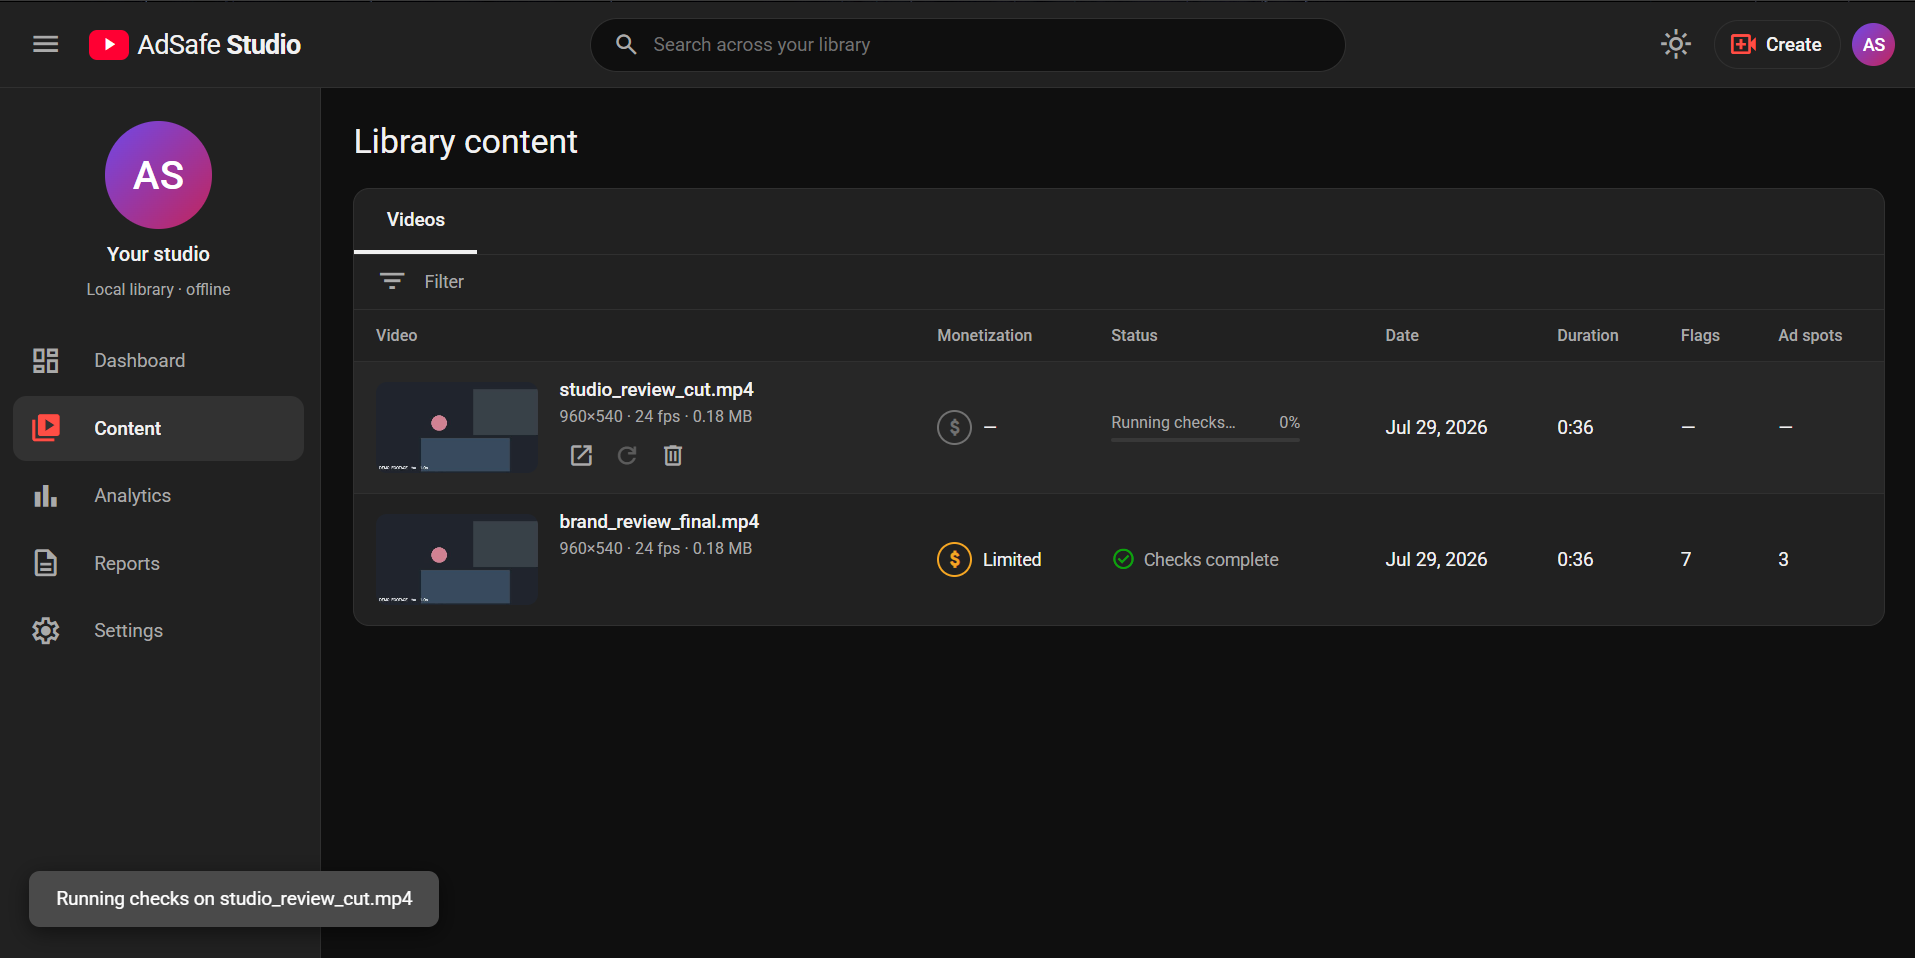
\includegraphics[width=\textwidth]{08-progress.png}
\caption{Analysis in progress. The status cell reports the active pipeline stage and
completion percentage, updated continuously without a page reload.}
\end{figure}

\begin{figure}[htbp]
\centering
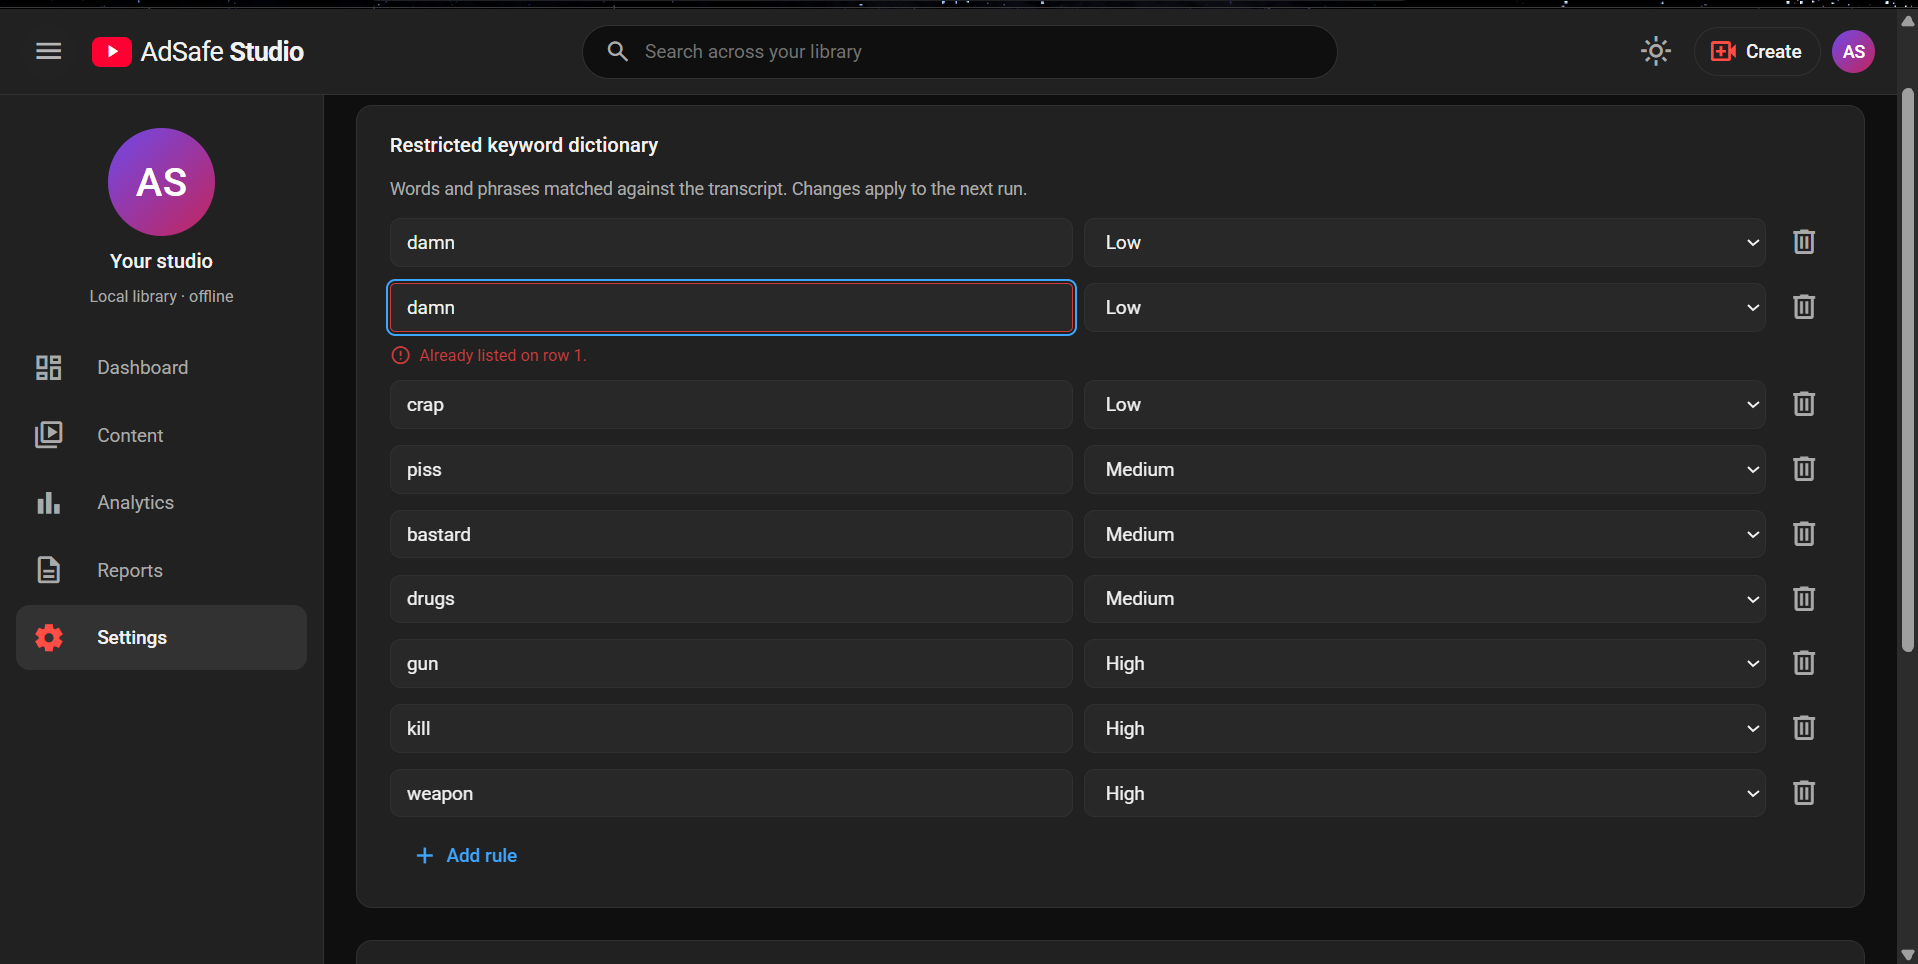
\includegraphics[width=\textwidth]{09-validation.png}
\caption{Inline validation. A duplicate dictionary entry is identified against the
offending field, and the Save action is disabled until it is resolved.}
\end{figure}

\clearpage

\begin{figure}[htbp]
\centering
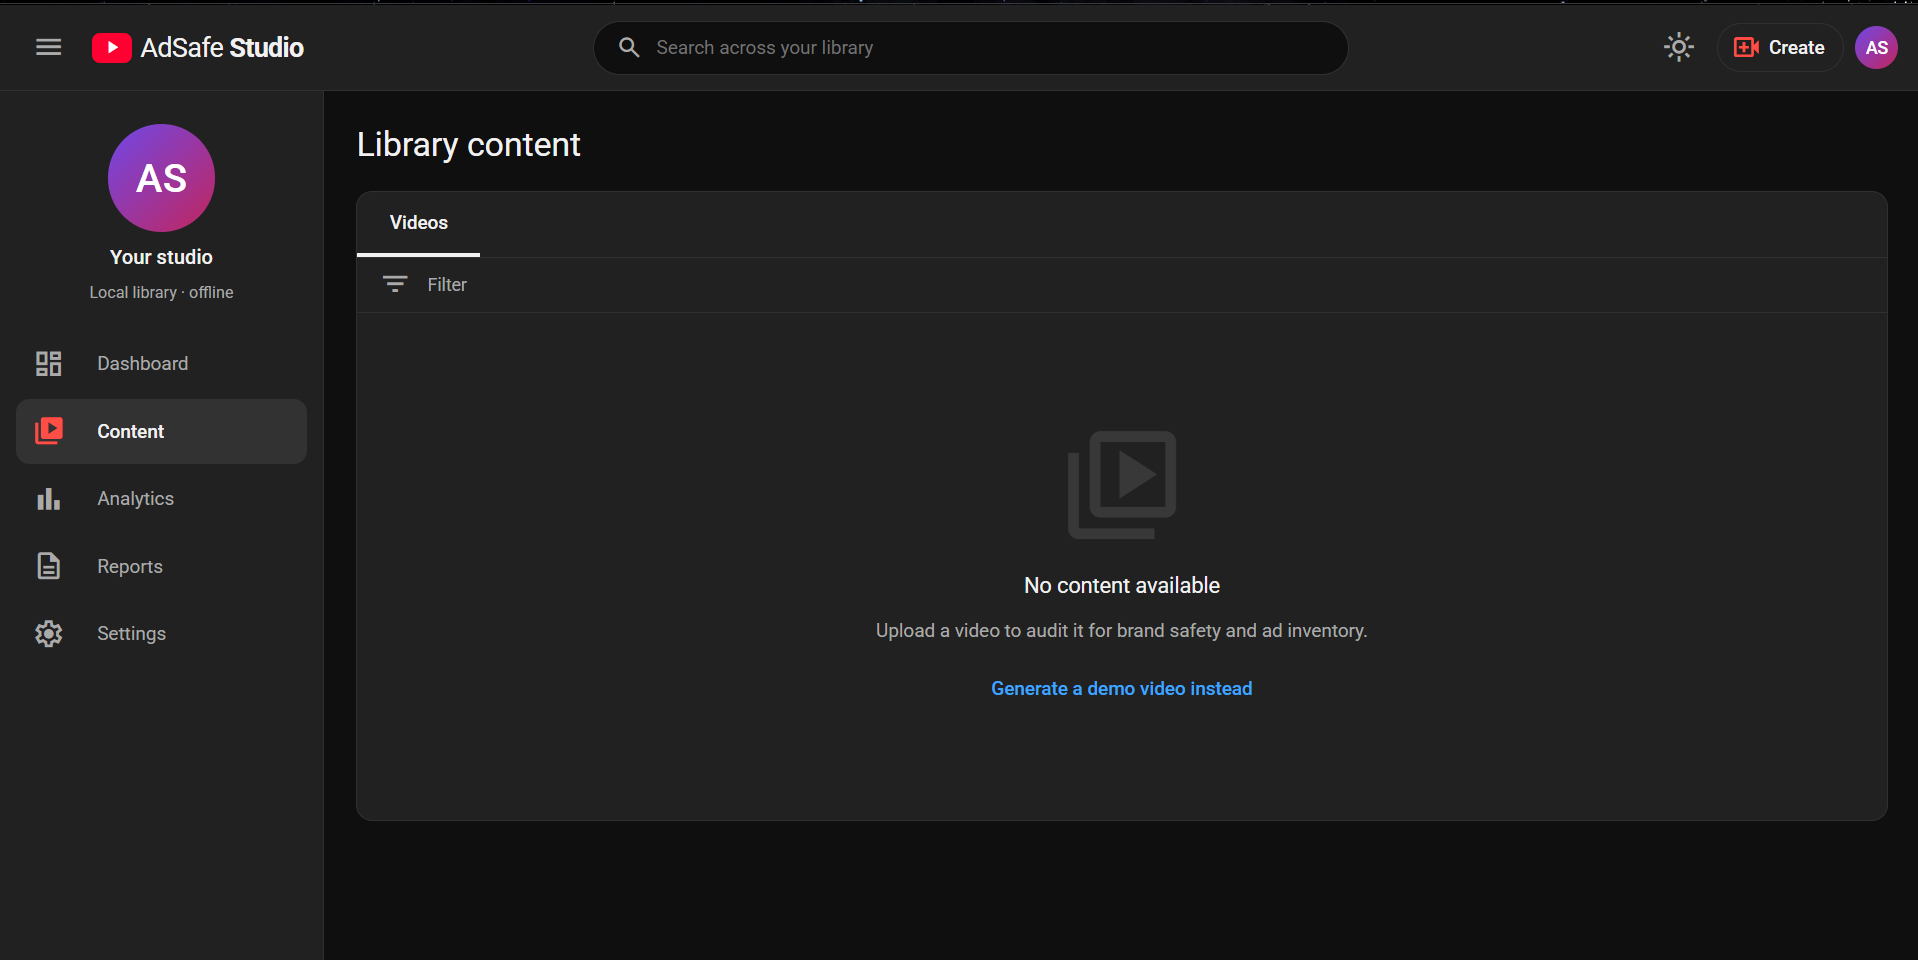
\includegraphics[width=\textwidth]{10-empty-state.png}
\caption{Empty state. Rather than presenting a blank table, the screen explains the
situation and offers the next action.}
\end{figure}

%%%%%%%%%%%%%%%%%%%%%%%%%%%%%%%%%%%%%%%%%%%%%%%%%%
\section{Field Validation Rules}
%%%%%%%%%%%%%%%%%%%%%%%%%%%%%%%%%%%%%%%%%%%%%%%%%%

Validation is enforced in the interface before submission, and again on the server.
Errors are reported inline, adjacent to the field responsible, and the corresponding
submit action is disabled while any error is outstanding.

\begin{longtable}{|p{3.6cm}|p{2.6cm}|p{6.4cm}|}
\hline
\textbf{Field} & \textbf{Type} & \textbf{Validation Rule}\\
\hline
\endhead
Video file & File picker & Mandatory. Extension must be \texttt{.mp4}, \texttt{.mov} or
\texttt{.avi}; file must be non-empty and at most 2048\,MB; must be a decodable video
stream\\
\hline
Restricted term & Text & Mandatory; leading and trailing whitespace trimmed; must be
unique within the dictionary (case-insensitive)\\
\hline
Term severity & Dropdown & Mandatory; one of Low, Medium, High\\
\hline
Frame sample rate & Number & Mandatory; numeric; range 0.25--4.0 frames per second\\
\hline
Minimum spot persistence & Number & Mandatory; numeric; range 2.0--15.0 seconds\\
\hline
Confidence threshold & Number & Mandatory; numeric; range 0.00--1.00\\
\hline
Transcription model & Dropdown & Mandatory; one of the supported model sizes\\
\hline
Report source video & Dropdown & Mandatory; restricted to videos whose analysis has
completed\\
\hline
Report format & Dropdown & Mandatory; one of CSV, JSON\\
\hline
Library search & Text & Optional; free text; filters the table as typed\\
\hline
\end{longtable}

%%%%%%%%%%%%%%%%%%%%%%%%%%%%%%%%%%%%%%%%%%%%%%%%%%
\section{Responsive Design}
%%%%%%%%%%%%%%%%%%%%%%%%%%%%%%%%%%%%%%%%%%%%%%%%%%

The interface adapts across four breakpoints. The layout is fluid between them; the
breakpoints mark where the structure itself changes.

\begin{table}[htbp]
\centering
\begin{tabular}{|p{2.4cm}|p{2.4cm}|p{7.6cm}|}
\hline
\textbf{View} & \textbf{Width} & \textbf{Adaptation}\\
\hline
Desktop & $\geq$1200\,px & Full navigation rail; two-column detail layout; four
statistic cards per row\\
\hline
Laptop & 900--1199\,px & Navigation collapses to an icon rail; detail layout becomes
single column; statistics two per row\\
\hline
Tablet & 600--899\,px & Navigation becomes an overlay drawer with a dimming scrim,
opened from the menu control; content spans full width\\
\hline
Mobile & $<$600\,px & Data table re-renders as a card list; search collapses; actions
become icon-only; statistics two per row\\
\hline
\end{tabular}
\end{table}

\begin{figure}[htbp]
\centering
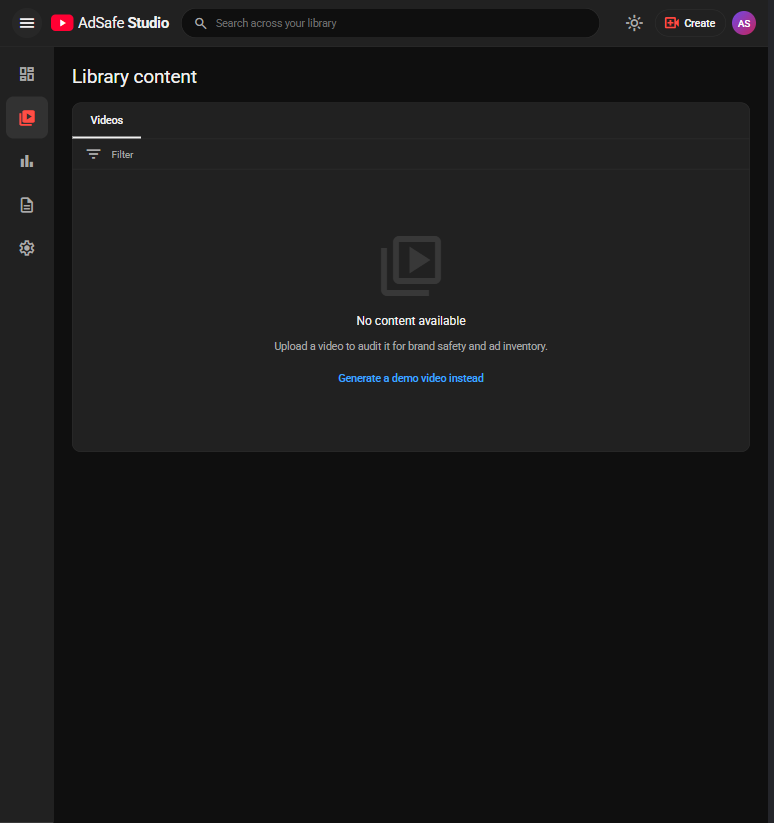
\includegraphics[width=0.78\textwidth]{11-responsive-laptop.png}
\caption{Laptop view --- navigation collapsed to an icon rail}
\end{figure}

\begin{figure}[htbp]
\centering
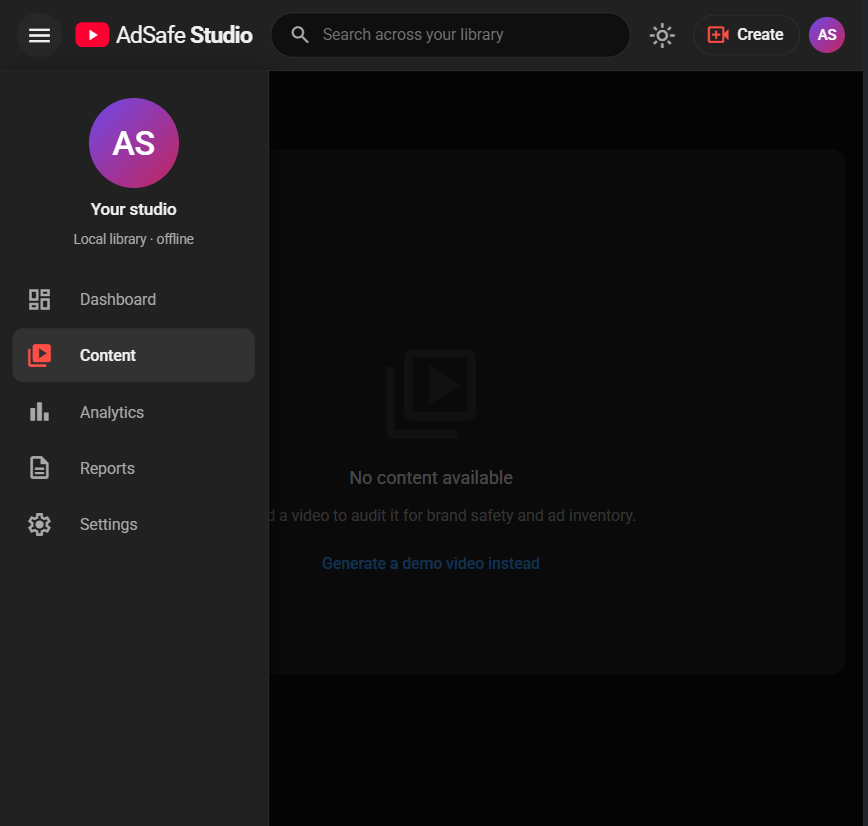
\includegraphics[width=0.62\textwidth]{12-responsive-tablet.png}
\caption{Tablet view --- navigation presented as an overlay drawer}
\end{figure}

\clearpage

\begin{figure}[htbp]
\centering
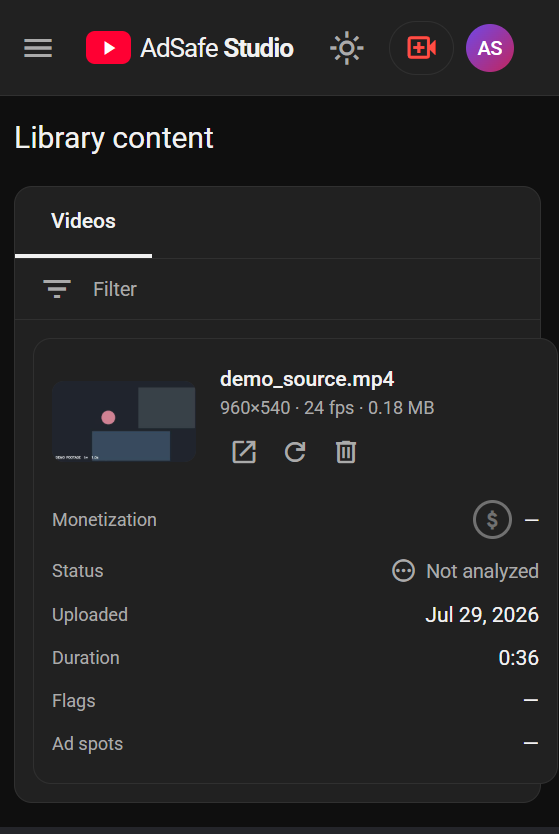
\includegraphics[width=0.42\textwidth]{13-responsive-mobile.png}
\caption{Mobile view --- the content table re-rendered as labelled cards. A horizontally
scrolling table is unusable at this width, so each row becomes a self-contained card
with its column headings restated as field labels.}
\end{figure}

%%%%%%%%%%%%%%%%%%%%%%%%%%%%%%%%%%%%%%%%%%%%%%%%%%
\section{Usability Considerations}
%%%%%%%%%%%%%%%%%%%%%%%%%%%%%%%%%%%%%%%%%%%%%%%%%%

\subsection{Consistency and Learnability}

\begin{itemize}[nosep]
\item A single persistent shell frames every screen, so navigation never relocates.
\item Severity colours, badge shapes, and status vocabulary are identical on every
screen where they appear.
\item The layout follows established creator-tool conventions, reducing the learning
required of the target user.
\end{itemize}

\subsection{Efficiency}

\begin{itemize}[nosep]
\item Every primary destination is one click from any screen.
\item Analysis runs in the background; the operator may navigate away and return.
\item Timeline events seek the player directly, removing manual scrubbing --- the
single largest time cost in manual review.
\item Reports are generated from the video being examined, without re-selecting it.
\end{itemize}

\subsection{Feedback and Error Prevention}

\begin{itemize}[nosep]
\item Long operations report a named stage and a percentage, never an indeterminate
spinner.
\item Destructive actions require confirmation.
\item Invalid input is identified against the field responsible, in plain language, and
blocks submission rather than failing afterwards.
\item Files are validated before upload begins, so a rejected file costs no transfer.
\item Empty states explain the condition and offer the next action.
\end{itemize}

\subsection{Accessibility}

\begin{itemize}[nosep]
\item Text contrast meets or exceeds WCAG~2.1 AA; interface components meet the 3:1
minimum. The action colour is themed specifically to satisfy this in dark mode.
\item Colour is never the only signal --- severity is always accompanied by a label.
\item The status palette is verified for colour-blind separation.
\item All controls are keyboard operable, including timeline events, and receive a
visible focus indicator.
\item Icon-only controls carry descriptive accessible names; status changes are
announced to assistive technology.
\item A closed navigation drawer is removed from the focus order.
\item Motion is suppressed for users who request reduced motion.
\end{itemize}

\subsection{Theming}

Both a dark and a light theme are provided; the preference persists between sessions
and is applied before first paint to avoid a flash of the wrong theme.

\begin{figure}[htbp]
\centering
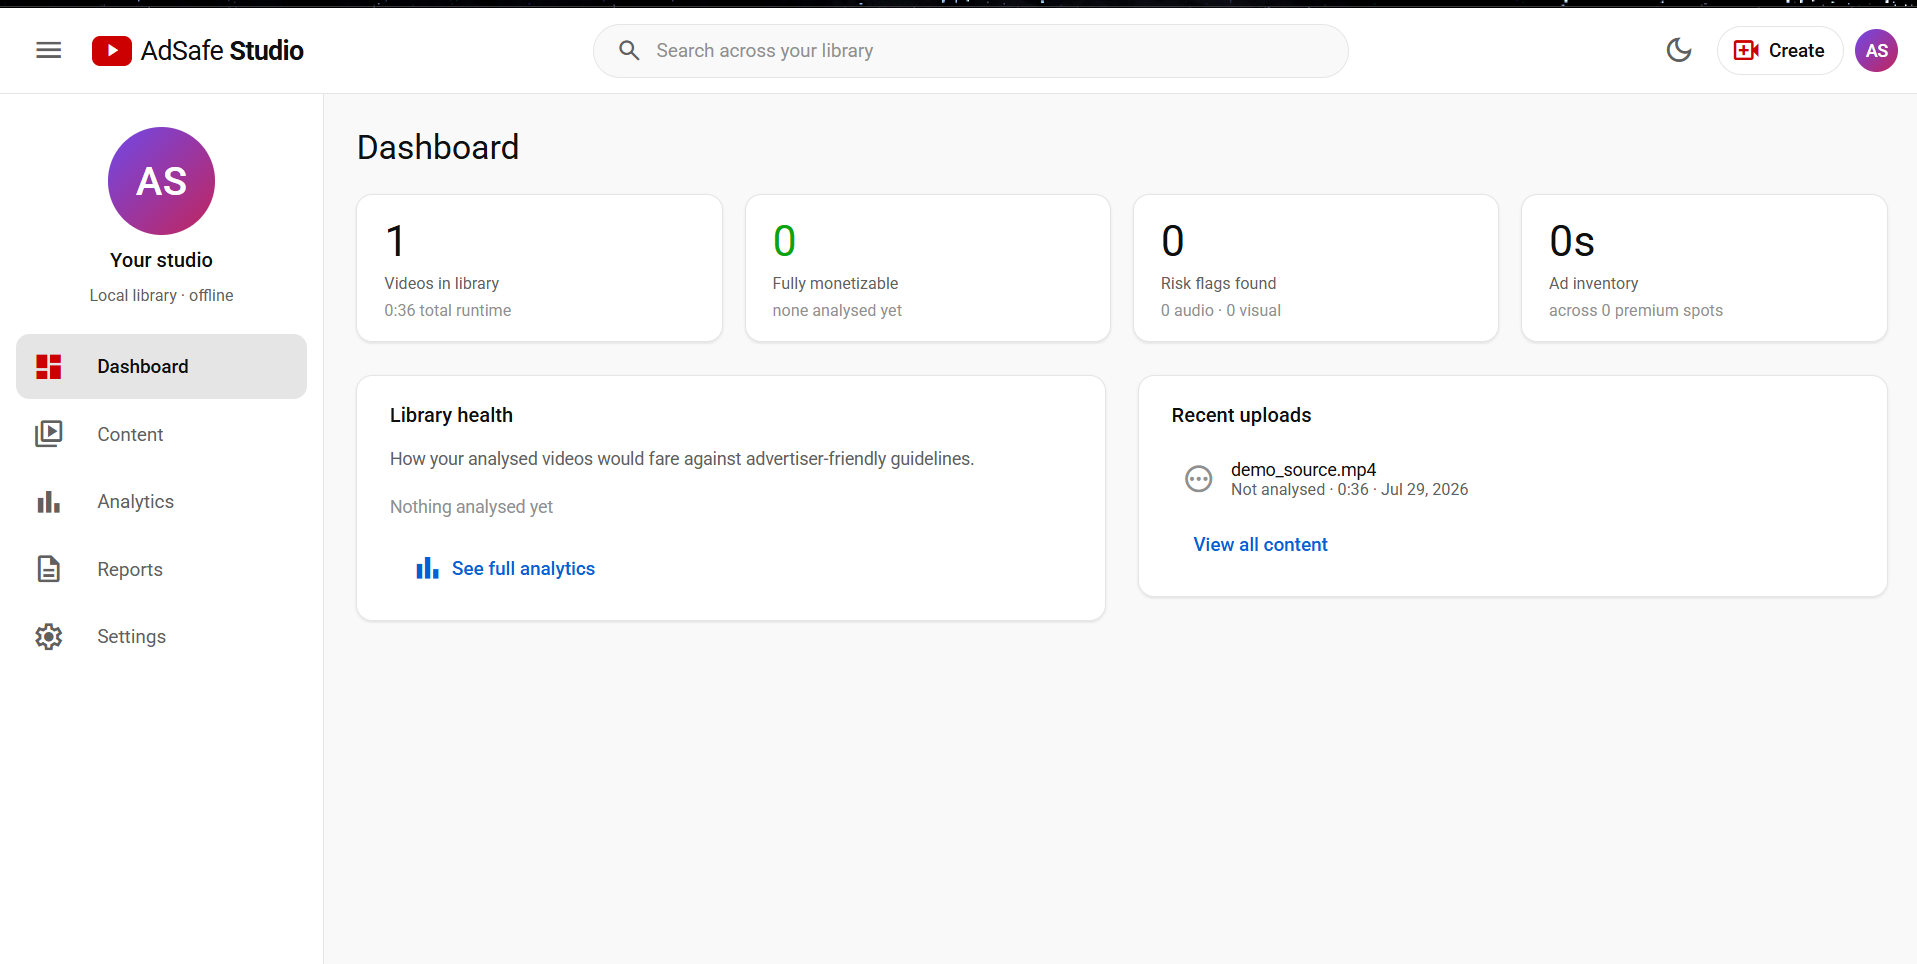
\includegraphics[width=\textwidth]{14-theme-light.png}
\caption{Light theme. Surfaces and text tokens invert; the action colour is substituted
to maintain contrast.}
\end{figure}

%%%%%%%%%%%%%%%%%%%%%%%%%%%%%%%%%%%%%%%%%%%%%%%%%%
\section{Prototype Screens}
%%%%%%%%%%%%%%%%%%%%%%%%%%%%%%%%%%%%%%%%%%%%%%%%%%

The high-fidelity prototype for this project is the \textbf{working application
itself}. Rather than producing static mockups in a design tool, the interface was
implemented directly and every figure in this document is a capture of the running
system.

\begin{table}[htbp]
\centering
\begin{tabular}{|p{4cm}|p{8cm}|}
\hline
\textbf{Item} & \textbf{Detail}\\
\hline
Implementation & React with Vite; custom design system in CSS\\
\hline
Interface served at & \texttt{http://localhost:8000}\\
\hline
Source repository & \url{https://github.com/meeeee21/autonomous-video-analyzer}\\
\hline
Prototype fidelity & Fully interactive; all navigation, validation, theming and
responsive behaviour is live\\
\hline
\end{tabular}
\end{table}

\noindent The prototype exceeds what a design-tool mock would demonstrate: the
navigation, validation, progress reporting, and responsive reflow shown in this
document are genuine behaviour rather than linked static frames.

%%%%%%%%%%%%%%%%%%%%%%%%%%%%%%%%%%%%%%%%%%%%%%%%%%
\section{Conclusion}
%%%%%%%%%%%%%%%%%%%%%%%%%%%%%%%%%%%%%%%%%%%%%%%%%%

This User Interface Design Document defines the visual design, navigation structure,
interaction behaviour, and validation rules of the Autonomous Video Ad-Placement \&
Contextual Safety Analyzer. Seven screens have been designed and implemented, spanning
four responsive breakpoints and two themes, with colour and contrast decisions verified
against measured accessibility criteria rather than chosen by appearance alone.

Because the interface is already implemented and operational, this document records a
realised design rather than a proposal. It serves as the reference for the remaining
implementation phases, during which the presentation layer stays fixed while the
underlying detection engines are completed.

%%%%%%%%%%%%%%%%%%%%%%%%%%%%%%%%%%%%%%%%%%%%%%%%%%
\section{Submission Checklist}
%%%%%%%%%%%%%%%%%%%%%%%%%%%%%%%%%%%%%%%%%%%%%%%%%%

\begin{enumerate}
\item User Interface Design Document (PDF) --- this document
\item Navigation Flow Diagram --- Section 3
\item Minimum Six Screen Wireframes --- Section 5, seven screens provided
\item High-Fidelity Prototype Screens --- Section 5, live application captures
\item Prototype Link --- Section 10, running application and source repository
\item Design Assets --- colour palette and typography specifications, Section 4
\end{enumerate}

\end{document}
